\documentclass[conference]{IEEEtran}

\usepackage{cite}
\usepackage[pdftex]{graphicx}
\usepackage[cmex10]{amsmath}
\usepackage{amssymb}
\usepackage{blindtext}
\usepackage[usenames, dvipsnames]{color}

\usepackage{hyperref}

\newcommand{\old}[1]{{}}
%\setlength{\parskip}{\baselineskip}%
\setlength{\parskip}{1.4mm}
%\usepackage[demo]{graphicx}
\usepackage[justification=centering]{caption}
\usepackage{subcaption}

\begin{document}
\title{Package Delivery with Trucks and Drones: The Horsefly Problem \vspace{-1ex}}
\author{
\IEEEauthorblockN{Joseph. S. B. Mitchell}
\IEEEauthorblockA{
  % Department of Applied Mathematics and Statistics\\
Stony Brook University}
% Stony Brook, NY 11794-3600 \\
% Email: joseph.mitchell@stonybrook.edu
\and
\IEEEauthorblockN{Gaurish Telang}
\IEEEauthorblockA{
  % Department of Applied Mathematics and Statistics\\
Stony Brook University}
% Stony Brook, NY 11794-3600\\
% Email: gaurish.telang@stonybrook.edu
}

\maketitle

\old{
  \begin{abstract}
Let $S=\{p_1,\ldots,p_n\}$ be a given set of $n$ customer sites in $\mathbb{R}^2$. A truck full of packages starts at point $s$ (the depot) and has a delivery drone on its rooftop. The drone can carry one package at a time to a customer, then return to the truck for another package.  The drone flies at speed 1, while the truck travels at (slower) speed $1/\varphi$, for a speed ratio $\varphi>1$.
The goal is to compute a route for the truck and for the drone in order to complete the delivery of all $n$ packages (and have the drone return back to the empty truck) as soon as possible -- i.e., we seek to minimize the {\em makespan} of the delivery process.
We describe algorithms to address this optimal delivery problem. We give both provable approximation results (an $O(\log n)$-approximation algorithm) and some experimental results comparing some heuristics.
\end{abstract}
}

\section{Introduction}

With recent advances in drone technology and their widespread
availability, several companies, including Amazon and UPS, have been
exploring the use of drones for delivering packages, potentially with
higher throughput at lower cost.  \textit{``UPS has estimated
  that cutting off just one mile for the routes of each of the
  company's 66,000 delivery drivers would amount to \$50 million in
  savings. For this reason, UPS is testing drone deliveries, using the
  top of its vans as a mini-helipad.''} \cite{dronepromise}. The video
in \cite{youtube} shows this concept in action.

We consider an optimal package delivery problem utilizing a truck and
a drone, specified as follows.  Let $S=\{p_1,\ldots,p_n\}$ be a given
set of $n$ customer sites in $\mathbb{R}^2$. A truck full of packages
starts at point $s$ (the depot) and has a delivery drone on its
rooftop. The drone can carry one package at a time to a customer, then
return to the truck for another package.  The truck moves at maximum
speed 1, while the drone flies at speed $\varphi\geq 1$; we refer to
$\varphi$ as the {\em speed ratio}.  The goal is to compute a route
for the truck and for the drone in order to complete the delivery of
all $n$ packages (and have the drone return back to the empty truck)
as soon as possible -- i.e., we seek to minimize {\em makespan} of the
delivery process.  We describe algorithms to address this optimal
delivery problem. We give both provable approximation results (an
$O(\log n)$-approximation algorithm) and some experimental results
comparing some heuristics.

The above problem has been called the \textit{Horsefly}
problem~\cite{john}.  It is easy to see that the Horsefly problem is
NP-hard, from the Euclidean TSP. (If the speed ratio $\varphi=1$, then
an optimal solution is for the drone and truck to travel together from
site to site on a TSP path.)
Figure~\ref{fig:example} shows an example of a routing for a truck and drone
for 30 sites, with $\varphi = 5$.

The challenge in computing a solution to the Horsefly problem is to
determine both the order of the sites in which they must be serviced
by the drone and the rendezvous points of the truck and the drone (the
points where the drone lands back on the truck to pick up the next
package, and then depart to the next customer).

It is also assumed in the above model that the truck itself cannot
make any deliveries: it is always the drone that must deliver a
package to every site. (The variant in which the truck/driver also
makes deliveries is also of interest but we defer that discussion to a
full paper.)

\old{
  The Horsefly problem is a direct generalization of the TSP-path problem: if 
\(\varphi = 1\), both the routes of the truck and the drone co-incide with
the TSP-path tour. Since the TSP itself is NP-hard, so is the horsefly problem.}

\begin{figure}
%\centering
\includegraphics[width=10cm]{img/prelim_example_phi5.png}
\caption{Delivery with truck and drone, with speed-ratio $\varphi=5$.
  The truck and drone travel along the red and green paths, respectively.
  The large red dot indicates the intial position $s$ of the truck and drone.}
\label{fig:example}
\end{figure}

\section{An $O(\log n)$ approximation algorithm}

\old{
  \begin{theorem}
  \label{thm:approx}
  The Horsefly problem in the plane has an $O(\log n)$-approximation algorithm.
\end{theorem}
}

The Horsefly problem in the plane has an $O(\log n)$-approximation algorithm.
%
We briefly sketch the proof.  The algorithm is based on computing, via
dynamic programming, a least expensive solution of a particular
structure: The truck traverses the edges of an orthogonal binary space
partition (BSP), while the drone's routes are doubled line segments
connecting each customer site $p_i$ to the closest point on the
boundary of the BSP face that contains it. The expense of a solution
is a weighted sum of the edge lengths: $\varphi$ times the total edge
length of the BSP network (the truck network), plus 1 times the
doubled segment lengths for the drone paths.  We argue that an optimal
solution to the Horsefly problem can be converted to a BSP-structured
solution at a cost of a factor $O(\log n)$ in the makespan. From the
optimal BSP-structured network, we can extract optimal routes for the
drone and truck, and a feasible delivery schedule, which must be
within factor $O(\log n)$ of optimal.

\section{Case: Delivery Order is Given}

We consider first the case in which the order in which customer sites
receive deliveries is given: $(p_1,p_2,\ldots,p_n)$.

We make some simple observations about the structure of an optimal solution:
\begin{description}
  \item[(1)] The truck route and the drone route are polygonal, with vertices
at a set of departure/rendezvous points, $s_1=s, s_2, s_3,\ldots,s_n$, where
point $s_i$ is a point along the truck route where the drone departs
to deliver the package to customer $p_i$. (And, thus, $s_i$ is also
the point on the truck route where the drone returns to the truck
after making the delivery to the customer at point $p_{i-1}$, for
$i\geq 2$.)
\item[(2)] The truck and the drone move always at their maximum speeds (1 and $\varphi$, respectively).
\end{description}

Given the ordering of the sites, the problem of computing the optimal
rendezvous points $s_i$ can be formulated as a convex program, which
can be solved by standard non-linear optimization solvers, such as the
Sequential Least Squares Programming (SLSQP) solver from \cite{slsqp},
which we use in our experiments. In order to speed up this
computation, we formulate the problem of computing optimal tours in
the $L_1$ (Manhattan) metric, which becomes a linear program.


\old{
% \subsection{Description of program}
% Make sure you mention the local optimiality property here which is useful. This actually
% helps you set up the constraints of the equation. 

We now sketch how the optimal route can computed \emph{if} the order of the delivery of the sites is given. Let the sites
be denoted \(S_i\)  and rendezvous points $P_i=(p_{2i-1}, p_{2i})$  for $1 \leq i \leq n$. Let \(P_0 = (\alpha,\beta)\)
denote the initial position of the truck and drone. Note that this initial position is given as part of the input.

We need to minimize the tour of the truck (the length of the red path in the figure above) by computing the appropriate
rendezvous points \(P_i\). The corresponding mathematical program is

$$\displaystyle \min_{(p_1,p_2,\ldots,p_{2n}) \in \mathbb{R}^{2n}}  \sum_{i=1}^{n}  || P_i - P_{i-1} ||$$

subject to the \(n\) constraints

$$|| P_{i} - P_{i-1} || = \frac{ || P_{i-1} - S_{i} ||   + || S_{i} - P_{i} ||  }{\varphi} \quad \text{for} \;\; i \in \{1,\ldots n\} $$

This problem can be easily solved by standard non-linear optimization solvers such as  the Sequential Least Squares Programming (SLSQP)
solver from \cite{slsqp} 

\subsection{A Linear Programming approximation}
   If the order in which the sites have to be visited is given then as described above
we can calculate the optimal tour using the SLSQP solver. However, the solver takes
a fairly long time to complete for even a small number of points. For instance it takes 
about a minute to run on a 100 sites. 

Here we describe a way to get an approximate tour using linear programming instead 
of the SLSQP solver, essentially using the $L1$ metric.  

\begin{figure}[h!]
\centering
\includegraphics[width=8cm]{img/lpdescr.pdf}
\end{figure}

Let the number of sites be \(n\) and let the \(i\) th site-coordinate be denoted by \((s_{2i}, s_{2i+1})\).
For each site, there is an associated triangle (shown in dark numbered circles in the figure above) where
the drone takes off from the truck, delivers the package to the site and returns to the truck. 

Let the initial position of the truck and drone be \((\alpha, \beta)\) and the rendezvous
points associated with the \(i\) th triangle be \((p_{2i-2}, p_{2i-1})\) and \((p_{2i}, p_{2i+1})\). 

We then solve the linear program $$\displaystyle \min \sum_{i=0}^{n} (h_{2i}+h_{2i+1})$$ subject to the following contraints
(Note that the constraints of the form $|a-b| \leq c$ split into two constraints $a-b < c$ and $-c \leq a-b$)


\begin{itemize}
\item Constraints associated with triangle \(0\) 
     \begin{align*}
0              &\leq f_{0}, f_{1}, h_{0}, h_{1} \\
| s_0-\alpha | &= b_0 \\ 
| s_1-\beta  | &= b_1 \\ 
\\
| p_0 - \alpha | &\leq h_0 \\
| p_1 - \beta  | &\leq h_1 \\
\\
| p_0 - s_0 | &\leq f_0 \\ 
| p_1 - s_1 | &\leq f_1 \\
\\
f_0 + f_1 + b_0 + b_1 &= \varphi h_0 + \varphi h_1
\end{align*}

\item Constraints associated with triangle \(i\) 
\begin{align*} 
0                       &\leq b_{2i}, b_{2i+1}, f_{2i}, f_{2i+1}, h_{2i}, h_{2i+1} \\
| s_{2i} - p_{2i-2} |   &\leq b_{2i}   \\ 
| s_{2i+1} - p_{2i-1} | &\leq b_{2i+1}   \\ 
| s_{2i} - p_{2i} |     &\leq f_{2i}   \\ 
| s_{2i+1} - p_{2i+1} | &\leq f_{2i+1}   \\ 
\\
| p_{2i} - p_{2i-2} |   &\leq h_{2i}   \\ 
| p_{2i+1} - p_{2i-1} | &\leq h_{2i+1}   \\ 
\\
f_{2i} + f_{2i+1} + b_{2i} + b_{2i+1} &= \varphi h_{2i} + \varphi h_{2i+1}
\end{align*}

\end{itemize}
}


Figure \ref{fig:lpslsqpcompare} is an example of the output of using SLSQP versus LP
obtained by the site-ordering given by the greedy heuristic for $\varphi=8$. Note that the
site \emph{orderings} are the same for both heuristics. (The ordering was
obtained using a greedy heuristic described in Section \ref{greedy}) The SLSQP based
method  took about 2 minutes to compute the tour whereas the LP based method
computed the tour in less than a second. Both times include the time taken
for computing the site ordering by the greedy heuristic

\begin{figure}
\centering
\begin{subfigure}[b]{0.55\textwidth}
  \includegraphics[width=0.8\columnwidth]{img/out1.pdf}
  \caption{Tour using SLSQP on site ordering  returned by \\ Greedy heuristic. Tour length 3.06500}
\end{subfigure}
\vspace{0.3cm}

\begin{subfigure}[b]{0.55\textwidth}
   \includegraphics[width=0.8\columnwidth]{img/out2.pdf}
   \caption{Tour using LP on site ordering returned by \\ Greedy heuristic: Tour Length 4.21343}
 \end{subfigure}
   \caption{An example of the tours computed via SLSQP and LP methods. Tour ordering computed via a greedy heuristic described in Section \ref{greedy}}
   \label{fig:lpslsqpcompare}
\end{figure}

\subsection{Comparing the exact and LP approximation ratio}

To test the approximation properties of the linear programming formulation, we compute the ratio of lengths of tours 
obtained via the LP heuristic and the exact SLSQP solver for different $\varphi$ on 100 uniformly distributed sites
in the unit square \([0,1]^2\). We then repeat the experiment 40 times. The initial position of the horse and drone
in all experiments was set to the middle of the square \((0.5,0.5)\). We used the MOSEK\cite{mosek} optimization
package for solving the resulting linear programs. 

The ratios of the tour lengths for each run and speed-ratio are plotted in the figure below, for various values of $n$ (horizontal axis).

\begin{figure}[h!]
\centering
\includegraphics[width=9cm]{img/tour_length_ratios.png}
\caption{ Comparing lengths of tours obtained from LP and SLSQP}
\label{fig:lpslsqp_expt}
\end{figure}

From Figure \ref{fig:lpslsqp_expt} it appears that the ratios of the tour-lengths is bounded for a
fixed-speed $\varphi$. Further the worst-case ratio seems to increase slowly
as a function of $\varphi$.
% We conjecture that this worst-case ratio grows asymptotically as  $\sqrt 2 \log \varphi$ (and $\sqrt d \log \varphi$ for general dimension $d$)


\section{Two heuristics}
% Put an example here with comparison for 100 points
% and a conjecture as to the approximation ratio
% achieved.
\subsection{Greedy Heuristic}
\label{greedy}

\begin{figure}[h!]
\centering
\includegraphics[width=6cm]{img/collinear_horseflies.png}
\caption{ The Collinear Horsefly problem }
\label{fig:collinear-horsefly}
\end{figure}

We first introduce a special case of the Horsefly problem, which we call {\em collinear-Horsefly}.
Here, the objective function is again to minimize the tour-length of the drone with
the additional restriction that the truck must always be moving in a straight line towards
the site on the line-segment joining itself and the site, while the drone is also
restricted to travelling along the same line segment. 
See Figure \ref{fig:collinear-horsefly} for an example instance of this problem, for $\varphi=3$.
With this additional restriction, the possible rendezvous points for the truck and the drone becomes finite. 
We show that an optimal (unrestricted) Horsefly solution can be converted to a collinear-Horsefly solution,
at a constant factor increase in the makespan.

\old{We hope to prove that for any drone speed \(\varphi\) the optimal horsefly tour can always be distorted by a 
constant factor \(D\) which is hopefully independent of (or at least a slowly growing function of)
of \(\varphi\) and the length of $OPT$ into a tour having the above structure for the same ordering of sites.
}

Similar to the nearest-neighbor insertion heuristic for the standard
TSP, a natural greedy strategy can be formulated for the
collinear-Horsefly problem; the truck always moves towards an
unvisited site nearest to its current position, while the drone takes
off from the truck, services the site, and flies back towards the
truck along the line joining the truck and the site again as shown in
\ref{fig:collinear-horsefly}.

\old{
  Since the problem of finding an optimal tour of the truck \emph{given}
the ordering of the sites can be solved optimally (using a convex
program in the $L_2$ case, or a linear program in the $L_1$ case), we
can use the ordering obtained from the greedy heuristic to compute a
better tour for the truck than the one obtained during the greedy
algorithm.}

Once the ordering of the sites is determined by the heuristic, we use
the fixed-ordering optimization program (using a convex program in the
$L_2$ case, or a linear program in the $L_1$ case) to compute the best
route for the truck (and thus for the drone), using the given
ordering.

\subsection{Clustering-Based Heuristic}

\begin{figure}[h!]
\centering
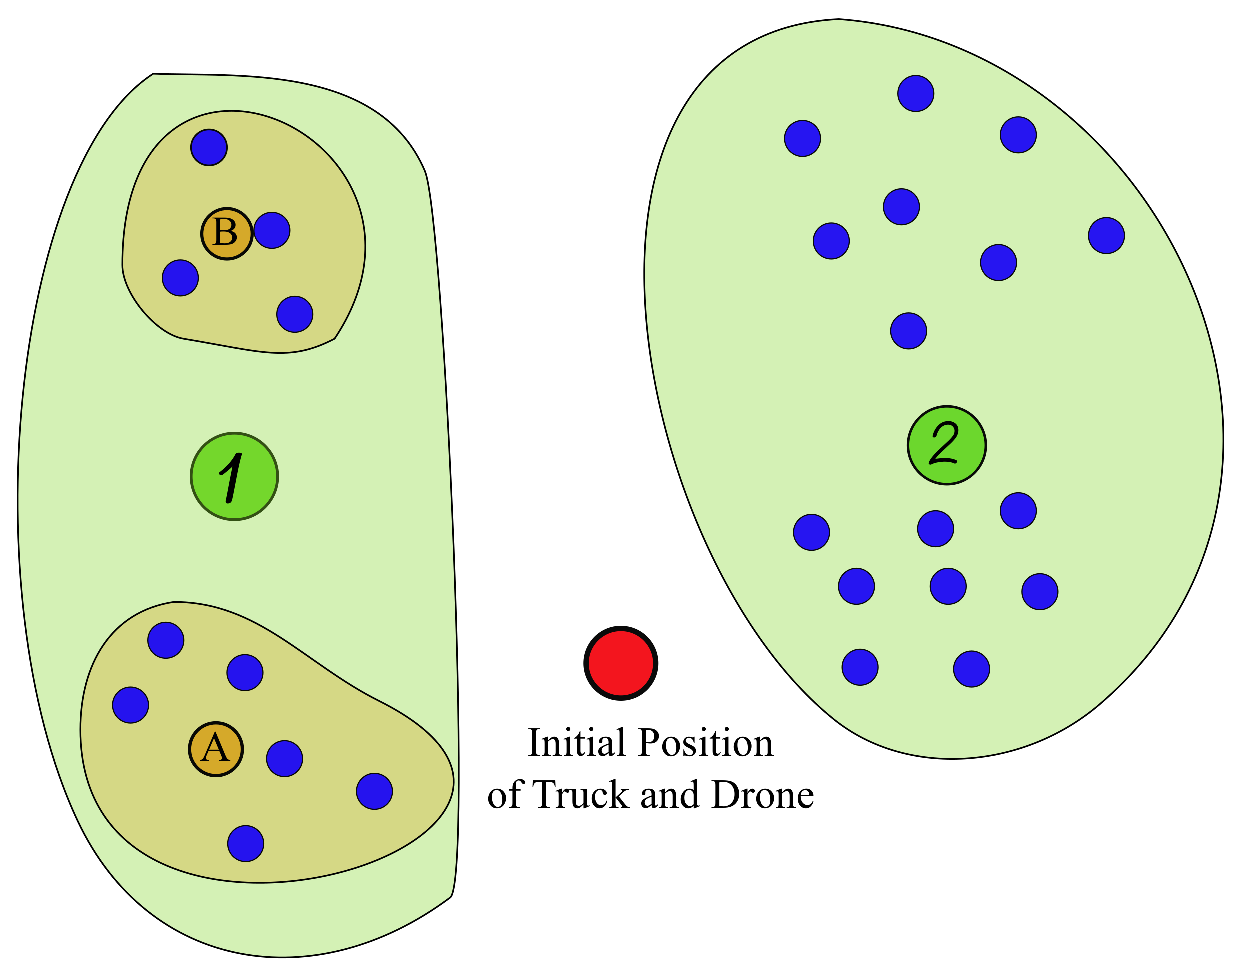
\includegraphics[width=5cm]{img/k2means_explain.eps}
\caption{The first two steps in the k2means heuristic for the Horsefly problem.}
\label{fig:k2means_explain}
\end{figure}

We describe another heuristic, which we call the ``k2means''
heuristic: Given the set $S$ of $n$ sites, we first compute the
2-centers along with associated cluster points for each of the
2-centers. We then use the exact algorithm to decide which center (and
hence cluster) to visit first.

In the above figure, for instance, we decide that the truck and drone
will coordinate to visit all of the sites in the left cluster first
and then the right. Within the chosen cluster, we again compute the
2-center and then use the exact algorithm for 2 points to decide which
sub-cluster should the truck and drone visit first. For instance, in
the example above, the heuristic decides to visit all the sites
associated with the 2-center \(A\) and then the
2-center \(B\).

We keep doing this recursively for each cluster, until we reach a
cluster size of 1 or 2.

In the above figure, once we finish visiting all of the sites in the
left cluster, we use the ending point of this subtour as the initial
point of the truck and drone to decide the order in which we must
visit the sites in the right cluster.

Once we finish calculating the order of the sites according to the
heuristic, we discard the computed path, and use the non-linear solver
to compute the optimal truck (and drone) path for this ordering.

% \newpage 
\subsection{An Example}

Figure \ref{fig:compareheuristics_example} compares two heuristics on one example of 100 sites distributed inside the unit-square, with $\varphi=8$. 

\begin{figure}[h!]
\centering
\begin{subfigure}[b]{0.55\textwidth}
  \includegraphics[width=0.8\columnwidth]{img/greedy_example.pdf}
  \caption{Tour obtained with the greedy heuristic.}
\end{subfigure}
\vspace{0.3cm}

\begin{subfigure}[b]{0.55\textwidth}
   \includegraphics[width=0.8\columnwidth]{img/k2means_example.pdf}
   \caption{Tour obtained with the k2means heuristic.}
 \end{subfigure}
\caption{An example of running the greedy and k2means heuristic on 100 sites}
\label{fig:compareheuristics_example}
\end{figure}


\subsection{Comparing tour-lengths for the two heurisitcs}

From Figure \ref{fig:compareheuristics}, we notice that the greedy heuristic
consistently outperforms the k2means heuristic by a slowly growing function
of $n$. The same behaviour was observed for other speed-ratios.

\begin{figure}[h!]
\centering
\includegraphics[width=8cm]{img/uniform_points/file_tour_lengths_00001.png}
\caption{Comparing the greedy and k2means heuristic}
\label{fig:compareheuristics}
\end{figure}


\begin{thebibliography}{1}
\bibitem{dronepromise}
   \textit{https://www.businessinsider.com/amazon-and-ups-are-betting-big-on-drone-delivery-2018-3}
\bibitem{youtube}
   UPS tests residential drone delivery. \textit{https://youtu.be/P5hQHBNpd7s}

 \bibitem{john}
   John Gunnar Carlsson, Siyuan Song
   \textit{Coordinated Logistics with a Truck and a Drone} 
   Management Science, 2017, \textit{https://doi.org/10.1287/mnsc.2017.2824}

\bibitem{mincostdrone}
  Ha, Q. M. and Deville, Y. and Pham, Q. D. and H{\`a}, M. H.
  \textit{On the Min-cost Traveling Salesman Problem with Drone},
  \textit{arXiv preprint arXiv:1512.01503}, 2015
\bibitem{campbell2017strategic}
  Campbell, James F and Sweeney, DC and II, Zhang J,
  \textit{Strategic design for delivery with trucks and drones}
  Technial Report, 2017
\bibitem{chao2002tabu}
  Chao, I.M.
  \textit{A tabu search method for the truck and trailer routing problem}
  Computers \& Operations Research, Elsevier  2002 volume 29, number 1, pages 33-51

\bibitem{slsqp}
  \href{https://docs.scipy.org/doc/scipy/reference/optimize.minimize-slsqp.html}{https://docs.scipy.org/doc/scipy/reference/optimize.minimize-slsqp.html} 

\bibitem{mosek}
  \href{https://www.mosek.com/}{https://www.mosek.com/}
  
\bibitem{scikit}
  \href{http://scikit-learn.org/stable/modules/generated/sklearn.cluster.KMeans.html}{http://scikit-learn.org/stable/modules/generated/sklearn.cluster.KMeans.html}


  
\end{thebibliography}
\end{document}

